\documentclass[../main.tex]{subfiles}

\begin{document}
\subsection{Alternative solutions and tradeoffs}
\begin{table}[H]
        \centering
	\caption{A comparison of the alternative solutions.}
        \label{tab:alt-solutions}
	\begin{tabular}{ p{4cm} p{6cm} p{6cm} }
		\toprule
		\textit{} & \textit{Design A} & \textit{Design B}\\ \midrule
		Type  & custom made drone with onboard computer & commercial drone with high performance and many features    \\
		Flexibility & very flexible and and customization is easy & hard to customize or modify it since it flies under limited protocols and standards. \\
		
		Price \& Availability & cheaper but the shipping and building processes must be considered & expensive but in our case its available in our hands and ready to fly.   \\
		
		Onboard computer & must have & must have \\
                \bottomrule
	\end{tabular}
\end{table} 
From the above table, we can see some tradeoffs between design A and design B, but in both designs, an onboard microcomputer must be present for flying control and the support of autopilot feature. There are three options for onboard microcomputers, which are shown in the following table. Raspberry Pi 4 seems to be the winner since it has advantages in specifications, connection interfaces, and availability.
\begin{table}[H]
        \centering
	\caption{A comparison of the onboard computers.}
        \label{tab:onboard-computers}  
	\begin{tabular}{ p{3cm} p{4cm} p{4cm} p{4cm} }
		\toprule
		\textit{} & \textit{Raspberry Pi 4} & \textit{NVIDIA Jetson Nano} & \textit{dji Manifold}\\ \midrule
		Specifications  & CPU:Cortex-A72 (ARM v8) 64-bit@ 1.5GHz | Ram :4GB or 8GB LPDDR4-3200 SDRAM | GPU : Broadcom VideoCore VI & CPU:Quad-core ARM A57 @ 1.43 GHz | Ram: 4 GB 64-bit LPDDR4   | GPU:128-core Maxwell & CPU:Quad-core,ARM | Ram: 2 GB DDR3L | GPU:Low-power GeForce graphics processor \\ \addlinespace
		Connection interfaces & 2.4 GHz and 5.0 GHz IEEE 802.11ac wireless, Bluetooth 5.0 & Gigabit Ethernet \& M.2 Key E (for WiFi support). &10/100/1000 BASE-T Ethernet \\ \addlinespace
		
		Price \& Availability & 300 QAR available and can be used on any drone & 400 QAR available but need to be ordered and shipped & very expensive and restricted to dji drones and dji company stopped selling it \\ \addlinespace
		Picture & \begin{minipage}{.2\textwidth}.
			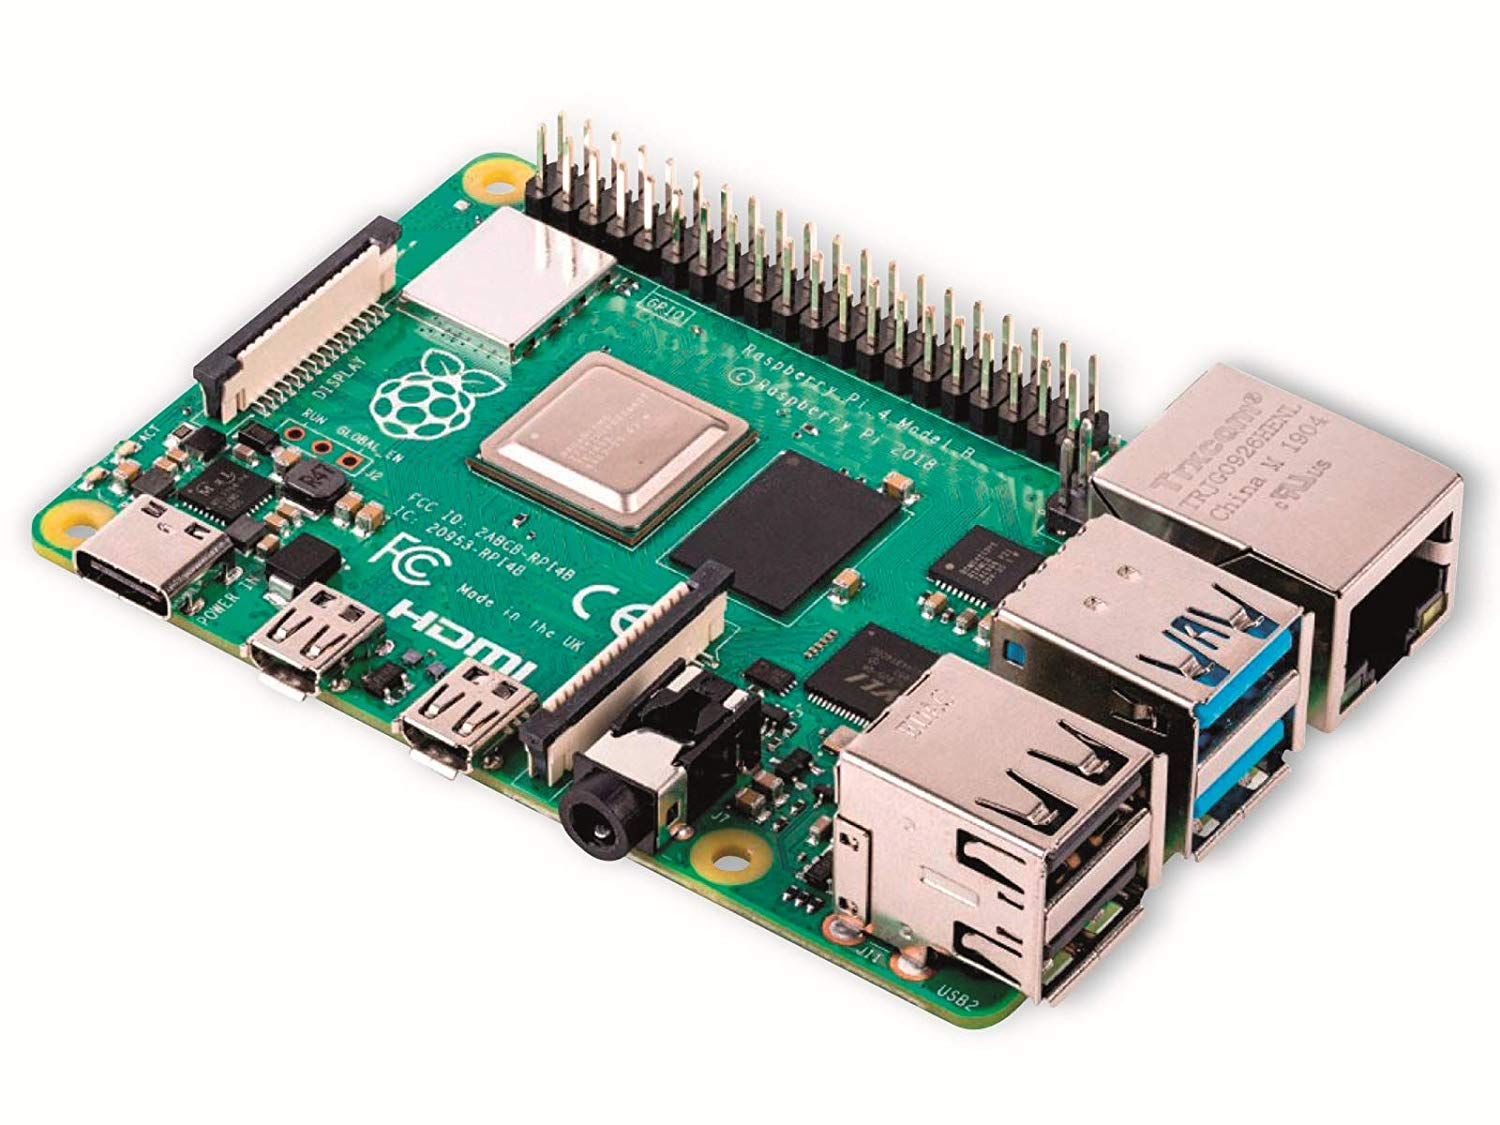
\includegraphics[width=40mm, height=30mm]{raspberry.jpg}
		\end{minipage}  & \begin{minipage}{.2\textwidth}.
		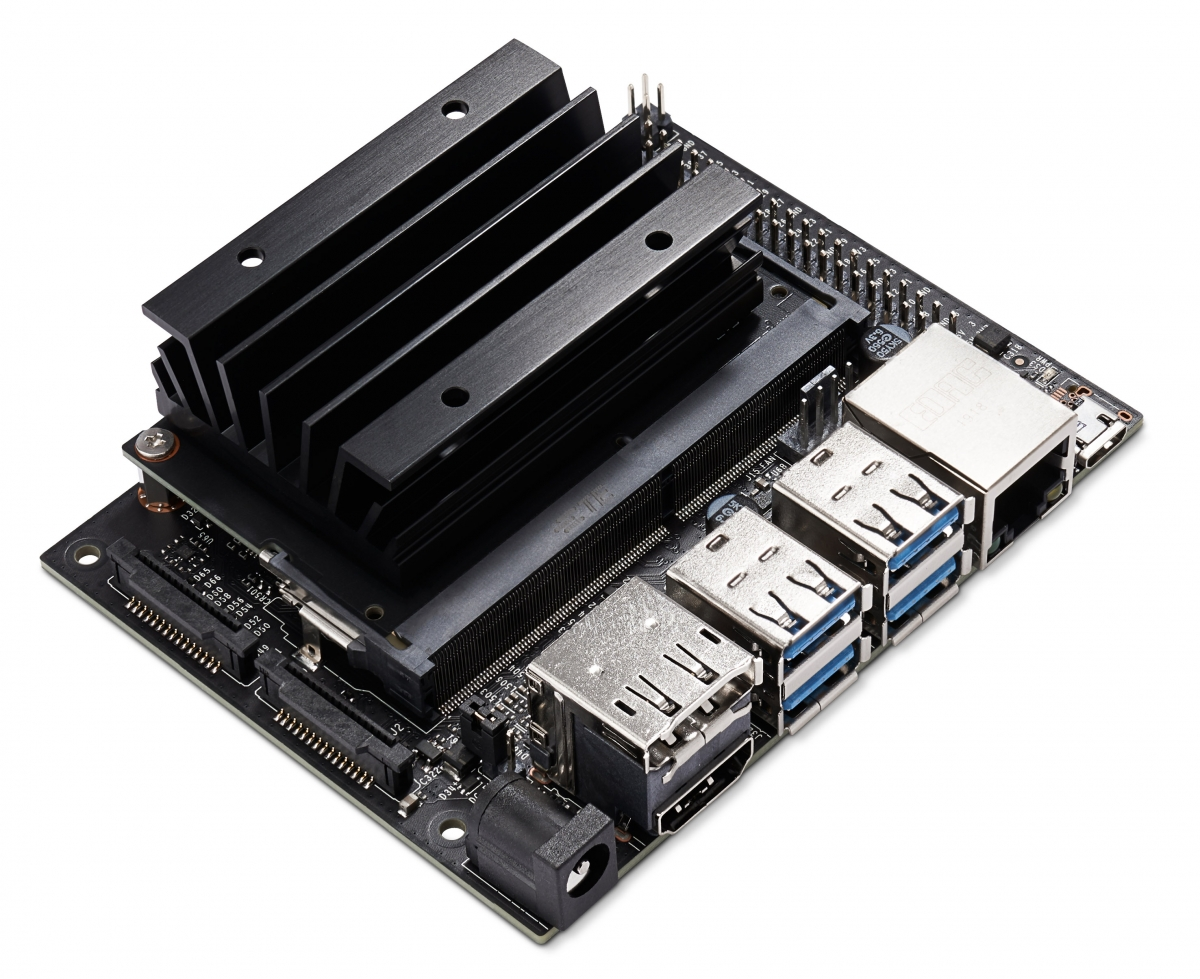
\includegraphics[width=40mm, height=30mm]{jetson.jpg}
	\end{minipage} & \begin{minipage}{.2\textwidth}.
	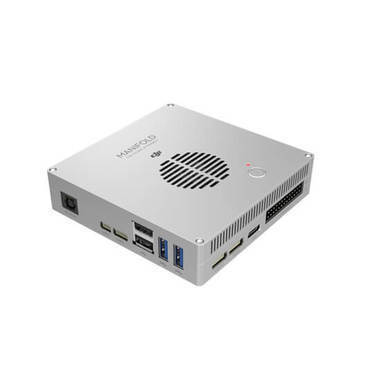
\includegraphics[width=40mm, height=30mm]{manifold.jpg}
\end{minipage} \\
            \bottomrule
	\end{tabular}
\end{table}
\newpage
\subsection{Selected solution overview}
The proposed solution consists of two main sections: a commercial drone and a controlling section.
We have chosen the commercial drones especially the Parrot \textsc{anafi} drone for several reasons.
Firstly, the support of SDK and the fluent control of the drone with a simple python script.which makes controlling the drone and moving it using \gls{drl} model much easier. 
Secondly, good flight time support as the \textsc{anafi} drone has 2700 mAh battery, it can fly up to 25 minutes which is good enough for our application.
Finally, the support of Wi-Fi 802.11 and \gls{gps} features is essential in our project for executing scripts and navigation. 
For how the system will work firstly, the user will import or choose the mobility pattern and set the constraints to the monitor device, which is a laptop.
Then the laptop will send high-level commands to the drone agent, which will apply certain operations such as start/stop etc.
Once the user finishes importing the mobility pattern and starting the drone mission, the drone will take off and begin visiting areas and scanning for the most number of mobile targets using \gls{drl} model.
Users will keep receiving live updates and the status of service on the control section using Wi-Fi.
Most of the connections in the system are wireless, which will have benefits and drawbacks  which are discussed in the hardware/software section.

\newpage
\subsection{High level architecture}
Figure ~\ref{fig1:arch-fig} shows a high-level architecture of a complete working system, in which a group of connected adapters and devices are combined into a single functional system. The architecture is composed of three sections, interfacing, controlling, and targets. The interfacing section contains the drone that will handle the onboard computer, its power source, and the connection adapters. In the controlling part, a personal computer will be responsible for contacting the onboard computer to adjust settings, execute scripts, and get live updates or results. Finally, there will be multiple moving targets in the target section. For example, R/C cars are controlled manually and moving in a specific mobility pattern with different directions and destinations. In the next section, hardware and software components will be presented in a more detailed way.

\begin{figure}[H]
	\centering
	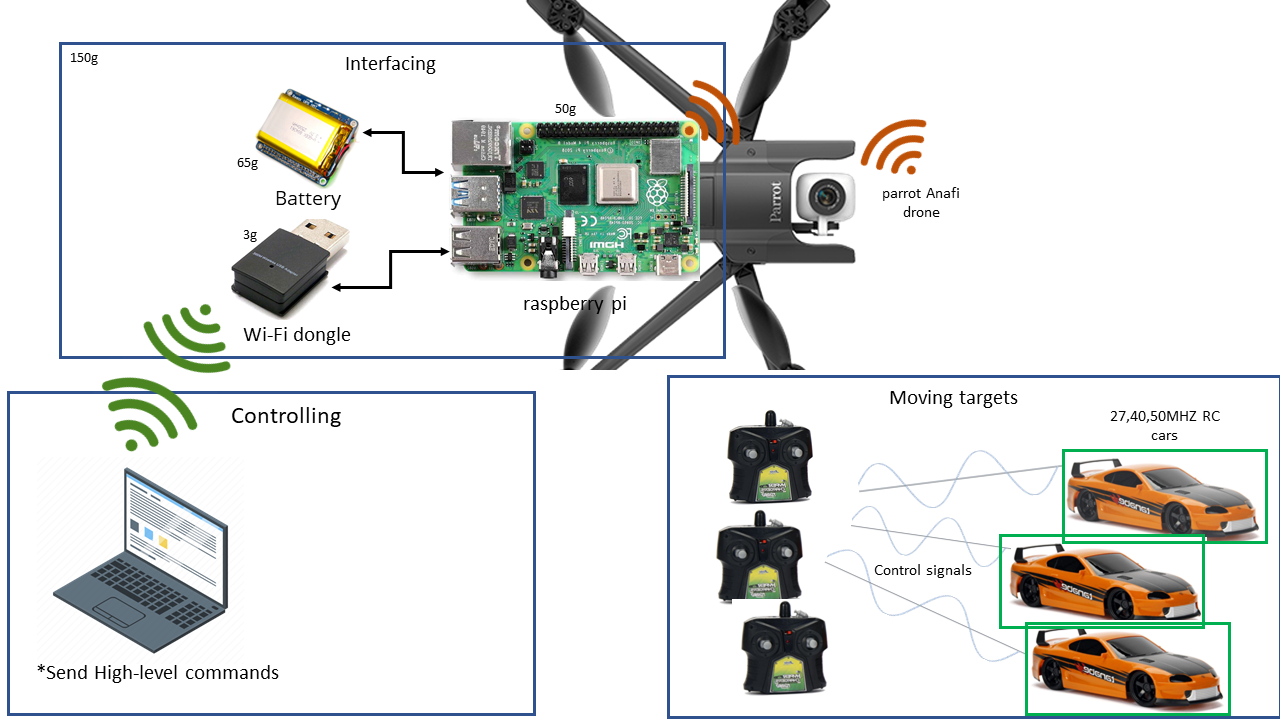
\includegraphics[width=0.9\textwidth]{high-level-arch.png}
	\caption{High-Level Architecture}\label{fig1:arch-fig}
\end{figure}


\subsection{Hardware/software to be used}

\subsubsection{Software}
%parrot olympe
%parrot sphinx
%Gazebo simulator
%roboflow
%google colab notebook /jupyter notebook
There are three primary categories of software depending on the usage: simulation, training, and application. The first part will focus on simulating the environment, testing the models, and flight control. Before discussing the software to be used, we have selected Ubuntu 18.04 as an operating system for several reasons. One key reason is the compatibility because parrot Olympe and Sphinx are only supported on limited distributions and operating systems. Another reason its a lite os and can be installed on the onboard computer that will be attached to the drone. For the simulation part, using Sphinx and Gazebo software is a very helpful tool to visualize the environment, control the drone, and apply \gls{drl} model. Sphinx is a simulation tool to run the Parrot drone firmware on personal computers, which comes with helpful features for simulation like visualizing flight data at runtime, running the \gls{uav} remotely, and executing scripts with the command line. Gazebo is a robot GUI simulation which simulates the visual and physical surrounding of drones and custom 3D objects. Figure ~\ref{fig2:gazebo} shows how the Gazebo and Sphinx look like. \begin{figure}[H]
	\centering
	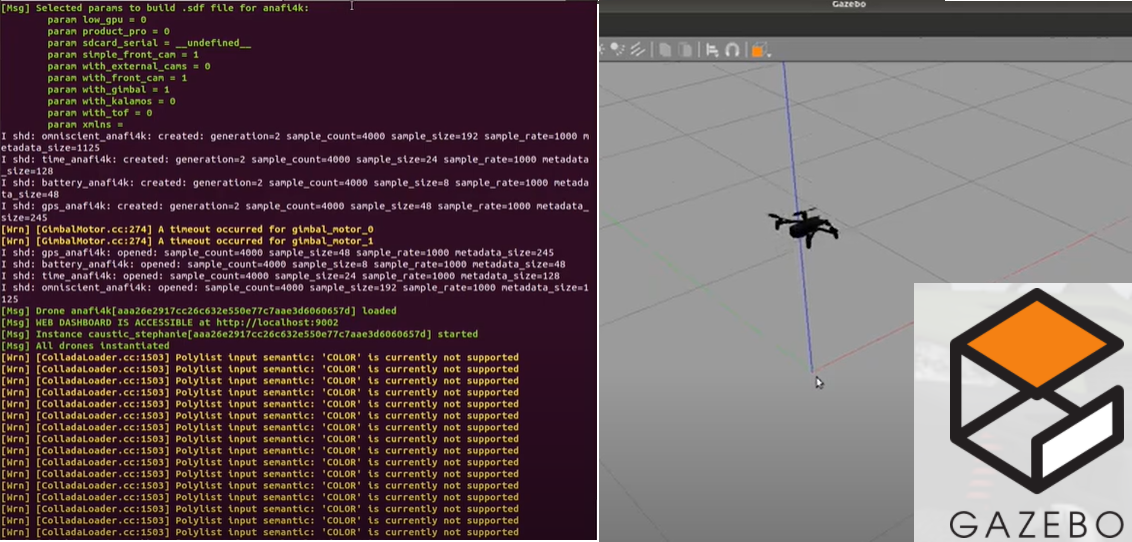
\includegraphics[width=0.6\textwidth]{gazebo.png}
	\caption{Sphinx and Gazebo }\label{fig2:gazebo}
\end{figure}
In the training part, we used simulation tools to generate some training datasets. Firstly, we placed random objects and captured the images using the simulated drone camera. We have used a website called roboflow which helped us labeling the objects and generate new datasets from the existing ones with modified constraints like rotation and scaling. For the object detection model, google colab notebook was a sufficient tool to start training using \gls{cnn} \textsc{yolo}v5, also Jupyter notebook was very helpful in executing demos. For the application software used parrot Olympe was used to send commands to the drone and control the flight trip and how the drone moves. Parrot Olympe uses Python controller programming interface for Parrot Drones which will make controlling simple and easy using a python script.


\subsubsection{Hardware}
%Parrot ANAFI Drone
%Raspberry Pi 4
%lithium Battery
%Wi-Fi adapter dongle
%laptop control station
The main core of the hardware part is the drone, which will be the Parrot \textsc{anafi} drone. This one has got a couple of features that made us choose it which has been listed in the Selected solution overview section. The second important device is the Raspberry Pi which will be used as an onboard computer and will handle several tasks such as connecting to the drone using a Wi-Fi interface. Controlling the drone by executing the python scripts to send/receive fly control instructions to the drone. Apply the machine learning and \gls{drl} models, which will be synchronized with the control part.Send/receive high-level commands and results to the laptop/pc ground station. It is connected using another 2.4GHz Wi-Fi interface with the help of a 300Mbps Wi-Fi adapter dongle connected to the Raspberry Pi through USB. The power source for the Raspberry Pi will be a lithium battery with a power board called UPSPack Standard Power Supply attached to the main Raspberry Pi board. It includes a 4000mAh lithium battery, which provides enough power and time for our application.the connection between the Raspberry Pi and the power board is shown in figure ~\ref{Fig3:connection}.
\begin{figure}[H]
	\centering
	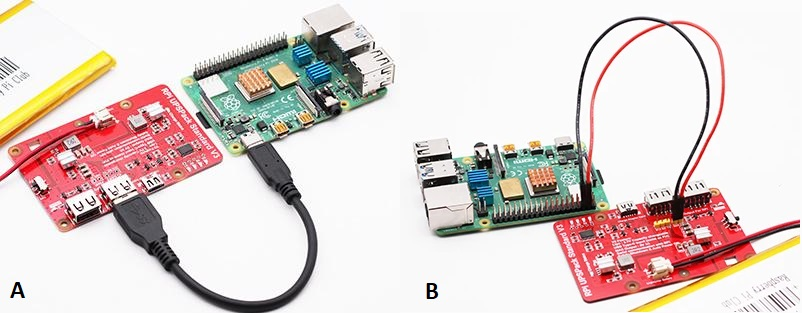
\includegraphics[width=0.6\textwidth]{connection.png}
	\caption{Raspberry Pi and Power board connection}\label{Fig3:connection}
\end{figure}     

\end{document}
